\documentclass[11pt]{article}
\usepackage{geometry}                % See geometry.pdf to learn the layout options. There are lots.
\geometry{letterpaper}                   % ... or a4paper or a5paper or ... 
%\geometry{landscape}                % Activate for for rotated page geometry
%\usepackage[parfill]{parskip}    % Activate to begin paragraphs with an empty line rather than an indent
\usepackage{graphicx}
\usepackage{amssymb}
\usepackage{epstopdf}
\usepackage{url}
\usepackage{slashbox}
\DeclareGraphicsRule{.tif}{png}{.png}{`convert #1 `dirname #1`/`basename #1 .tif`.png}

\title{A Flexible Method for Allocating, Learning, and Forgetting OpenLCB EventIDs}
\author{D.E. Goodman-Wilson\\Railstars\\dgoodman@railstars.com}
%\date{}                                           % Activate to display a given date or no date

\begin{document}
\maketitle
\begin{abstract}
OpenLCB Producer/Consumer nodes require some method of storing the EventID's to which they respond. One method uses a simple array of EventIDs, the position of which indicates to which producer or consumer the EventID is assigned. This method has the benefit of simplicity and compactness, but with two distinct costs. First, each producer or consumer is limited to producing or consuming exactly one EventID, reducing the flexibility. Second, Duplicate EventIDs are stored multiple times, reducing the general case space efficiency. In this paper, I discuss an alternate strategy for storing EventIDs in a matrix, in which each row represents an EventID, and each column represents a producer or consumer. This scheme is obviously more complex, but overcomes the two stated shortcomings, although at the cost of added time complexity for production of events.
\end{abstract}

\tableofcontents

\section{Motivation}

Simple consumer/producer schemes in which each producer or consumer is assigned exactly one EventID are sufficient for layouts in which there is a strict one-to-one, one-to-many, or many-to-one mapping of producers to consumers. However, achieving a many-to-many mapping requires that consumer or producers be able to consume or produce more than one EventID.\footnote{Much of this discussion, and indeed the algorithm described in the paper is derivative of the note at \url{http://openlcb.org/trunk/documents/notes/ProducerConsumerModel.html}.}

\begin{figure}[htbp]
\begin{center}
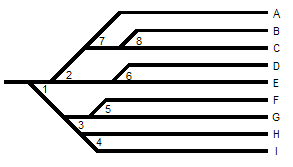
\includegraphics{CompoundLadder.png}
\caption{A compound yard ladder with turnouts 1--8 and routes A--I}
\label{ladder}
\end{center}
\end{figure}


For example, route selection through the yard ladder in Figure \ref{ladder}. In order to select the routes individually though a yard ladder, either the consumers attached to each turnout (especially the root turnout) must be able to respond to multiple events, or each control panel button must be able to send multiple events. For example, if each turnout responds to exactly one event, then pressing the button for \textit{A} must send multiple eventIDs, one each for turnout 1, 2, and 7. Alternately, if each button is configured to produce exactly one event, the turnout 1 must be configured to listen for multiple events, one for each button.

\section{Representation}

\subsection{Linear representation}

For a baseline, here is how EventIDs are stored in the current Producer/Consumer code in the C libraries of Bob Jacobsen, \textit{et al}, and of D.E. Goodman-Wilson. Assume $n$ producers and consumers; each is assigned a unique index from the range ${1,\ldots,n}$. We then create an EventID array of size $n$, as in Table \ref{linear}. Each cell in the array is of size(EventID); for $n$ producers/consumers, the storage requirements are thus size(EventID)$*n$.
\begin{table}[htdp]
\caption{Linear representation}
\begin{center}
\begin{tabular}{r|c|c|c|c|}
producer/consumer&0&1&$\cdots$&n \\ \hline
EventID&eid$_0$ & eid$_1$ & $\cdots$ &eid$_{n}$\\
\end{tabular}
\end{center}
\label{linear}
\end{table}%

\subsection{Two-dimensional representation}

One way to expand on this scheme to work for many-to-many transactions is to use a two-dimensional array of depth $m$, as in Table \ref{two-dim}, thus permitting each producer and consumer to take $m$ EventIDs.

Although this representational scheme does in fact increase the number of events that a producer or consumer can produce or consume, it does so inefficiently. First, consider that the storage requirements have increased to size(EventID)$*n*m$ bytes. Second, consider that many of the entries will sit unused.

Thus, in the yard ladder example in Figure \ref{ladder}, the root turnout \textit{1} must respond to nine possible route-selection-events, where the four leaf turnouts need only respond to one\footnote{Of course, each turnout has two consumers: One for straight, and one for diverging; But each of these consumers need only listen to one button each.}. Thus, because there are 8 turnouts, we need an array with 72 elements, which amounts to a staggering 576 bytes; and yet only 30 of these slots will actually be used. %TODO CHECK MY MATH!

\begin{table}[htdp]
\caption{Two-dimensional representation}
\begin{center}
\begin{tabular}{r|c|c|c|c|}
producer/consumer&0&1&$\cdots$&n \\ \hline
EventID 1&eid$_{0,0}$ & eid$_{0,1}$ & $\cdots$ &eid$_{0,n}$\\
EventID 2&eid$_{1,0}$ & eid$_{1,0}$ & $\cdots$ &eid$_{1,n}$\\
$\vdots$ & $\vdots$ & $\vdots$ & $\ddots$ & $\vdots$\\
EventID $m$ & eid$_{m,0}$ & eid$_{m,0}$ & $\cdots$ &eid$_{m,n}$\\
\end{tabular}
\end{center}
\label{two-dim}
\end{table}%

\subsection{Sparse matrix representation}

One obvious way forward, and the method I advocate in this paper, is to use a spare matrix to represent the producer/consumer--EventID pairings. Table \ref{matrix} presents such a sparse matrix, with each row representing one EventID, and each column representing one producer or consumer. Each cell, rather than representing an EventID, represents whether a the EventID at that row is to be connected to the producer or consumer at that column. This connection can be represented with just one bit of information, rather than the full 8 bytes required by an EventID. Thus, for $n$ producers and consumers, and $m$ distinct EventIDs, a sparse matrix requires only Size(EventID)$*m + (n*m)/8$ bytes, only marginally larger than the one-dimensional representation above.

A Sparse matrix has the further advantage of using this space efficiently. Increasing the available number of EventIDs by one for producers or consumers that require them entails a storage space increase of no more than size(EventID) +$n/8$ bytes. Looking again to the yard ladder example, with $m=9$ unique EventIDs required (one for each route), and $n=8$ producers (one for each turnout), the total space required is only $9*$size(EventID) $+ (9*8)/8 = $ a mere 81 bytes. Compare to the 576 bytes required above.

\begin{table}[htdp]
\caption{Sparse matrix representation}
\begin{center}
\begin{tabular}{c|c|c|c|c|}
\backslashbox{EventID}{producer/consumer}	&	0	&	1	&	$\cdots$	&	n \\ \hline
eid0				& $x_{0,0}$ & $x_{0,1}$ & $\cdots$ & $x_{0,n}$\\ \hline
eid1				& $x_{1,0}$ & $x_{1,1}$ & $\cdots$ & $x_{1,n}$\\ \hline
$\vdots$			& $\vdots$ & $\vdots$ & $\ddots$ &  $\vdots$  \\ \hline
eid\textit{m}		& $x_{m,0}$ & $x_{m,1}$ & $\cdots$ & $x_{m,n}$\\ \hline
\end{tabular}
\end{center}
\label{matrix}
\end{table}%

\subsection{Disadvantages of the sparse matrix representation}

Of course, there are costs to the sparse matrix representation. First, and most obviously, the representation can only contain $m$ unique EventIDs total, where the two-dimensional representation can represent a much larger number of unique EventIDs, $m*n$. Typically, this extra flexibility is not necessary, however, and the benefit is in the general case far outweighed by the inefficiency, especially on small microcontrollers with limited memory.

The second disadvantage is that the sparse matrix requires a rather high time-cost for determining which events to produce. If we know that producer $t$ has triggered, we must scan all $m$ rows of the sparse matrix to determine which EventIDs to use when sending out Producer/Consumer Event Reports (PCERs), when perhaps considerably fewer than $m$ EventIDs will be produced. Thus, the average time to generate the necessary PCERs is a constant $O(m)$. On the other hand, the two dimensional array can be sorted such that one need not scan through all $m$ entries, testing each in turn. If the columns are sorted such that genuine EventIDs are at the beginning, and empty place-holders are at the end, the on average the time to generate the necessary PCERs is $O(m/2)$ (and perhaps less, perhaps in many common cases as low as $O(\ln m)$).

Nevertheless, the space saving seen with the sparse matrix representation makes it a favorable choice for all but the simplest, most basic OpenLCB nodes.

\section{Learning}

Of course, these representations are not very useful unless we have some kind of learning algorithm with which to populate them. The sparse matrix representation requires a slightly different learning algorithm than the linear or two-dimensional representations. First, for comparison, let's look at the linear learning algorithm. (Because the linear and two-dimensional cases are largely the same, I will not cover the two-dimensional learning algorithm for the sake of simplicity.)

\subsection{Linear representation}

In the linear case, we require an additional bit attached to each EventID cell. This bit acts as a flag that tells the node what to do with the next received LearnEvent message---a learn flag. When a producer or consumer is selected for learning, a flag set at the cell at index $t$, which indicates that whatever EventID is located in the array at index $t$ is to be over-written by the EventID contained in the next LearnEvent message received. The total additional overhead is, for $n$ producers and consumers, $n/8$ bytes. The learn flag is then cleared.

\subsection{Sparse matrix representation}

Where the linear algorithm attaches a flag to each cell, learning in the sparse matrix attaches a bit to each column, that is, to each producer and consumer. When a producer or consumer is selected for learning, a flag is set for the entire column. The next received LearnEvent message will then trigger one of three actions. If there is a row that already contains the EventID contained in the LearnEvent message, then the bit at that column and row is set. If there is no row that already contains the EventID, and there is an empty row, then the EventID stored in the next empty row, and the bit at that column and row is set. Finally, if there is no free row, an out-of-memory condition of some kind is raised, and the LearnEvent is discarded.\footnote{Alternately, the new EventID might overwrite the oldest or least-recently-used EventID in the table, but this strategy requires, naturally, additional overhead.}

Here is a small example. We begin with an empty sparse matrix with four consumers, and four EventID rows, as in Table \ref{example1}. Empty EventID slots are indicated with $\emptyset$. In this state, none of the four consumers will consume any EventID.

\begin{table}[htdp]
\caption{Sparse matrix example, $t=0$}
\begin{center}
\begin{tabular}{c|c|c|c|c|}
producer/consumer	&	0	&	1	&	2	&	3 \\ \hline
\backslashbox{EventID}{learn flag}	&	0	&	0	&	0	&	0 \\ \hline
$\emptyset$ & 0 & 0 & 0 & 0 \\ \hline
$\emptyset$ & 0 & 0 & 0 & 0 \\ \hline
$\emptyset$ & 0 & 0 & 0 & 0  \\ \hline
$\emptyset$ & 0 & 0 & 0 & 0 \\ \hline
\end{tabular}
\end{center}
\label{example1}
\end{table}%

Suppose now that the user has selected consumer no. 2 to learn an EventID.\footnote{User interfaces for teaching EventIDs, such as the Blue/Gold algorithm, are outside the scope of this paper.} The node sets the learn flag for column 2, as per Table \ref{example2}.

\begin{table}[htdp]
\caption{Sparse matrix example, $t=1$}
\begin{center}
\begin{tabular}{c|c|c|c|c|}
producer/consumer	&	0	&	1	&	2	&	3 \\ \hline
\backslashbox{EventID}{learn flag}	&	0	&	0	&	1	&	0 \\ \hline
$\emptyset$ & 0 & 0 & 0 & 0 \\ \hline
$\emptyset$ & 0 & 0 & 0 & 0 \\ \hline
$\emptyset$ & 0 & 0 & 0 & 0  \\ \hline
$\emptyset$ & 0 & 0 & 0 & 0 \\ \hline
\end{tabular}
\end{center}
\label{example2}
\end{table}%

Now, when the user triggers a LearnEvent containing EventID eid$_0$, we scan the rows, and see that the EventID of none match the LearnEvent (because they are all empty). We pick one of the empty rows, and record the EventID at that row, and set the bit at that row for consumer 3.\footnote{If we always pick the first empty one, we can cut down on the time cost of this search, since we can always stop when we either hit the end of the list, or find an empty row.} The learn flag for consumer 2 is cleared. The result is Table \ref{example3}.

\begin{table}[htdp]
\caption{Sparse matrix example, $t=2$}
\begin{center}
\begin{tabular}{c|c|c|c|c|}
producer/consumer	&	0	&	1	&	2	&	3 \\ \hline
\backslashbox{EventID}{learn flag}	&	0	&	0	&	0	&	0 \\ \hline
eid$_0$ & 0 & 0 & 1 & 0 \\ \hline
$\emptyset$ & 0 & 0 & 0 & 0 \\ \hline
$\emptyset$ & 0 & 0 & 0 & 0  \\ \hline
$\emptyset$ & 0 & 0 & 0 & 0 \\ \hline
\end{tabular}
\end{center}
\label{example3}
\end{table}%

Suppose, finally, that the user wants to assign the same EventID to consumer 3. The user selects consumer 3 for learning, as per Table \ref{example4}, and then triggers a LearnEvent containing EventID eid$_0$ once again. We scan the rows, and this time see that the EventID at row 0 matches the LearnEvent. We set the bit at column 2, and clear the learn flag. The result is Table \ref{example5}.

\begin{table}[htdp]
\caption{Sparse matrix example, $t=1$}
\begin{center}
\begin{tabular}{c|c|c|c|c|}
producer/consumer	&	0	&	1	&	2	&	3 \\ \hline
\backslashbox{EventID}{learn flag}	&	0	&	0	&	0	&	1 \\ \hline
eid$_0$ & 0 & 0 & 1 & 0 \\ \hline
$\emptyset$ & 0 & 0 & 0 & 0 \\ \hline
$\emptyset$ & 0 & 0 & 0 & 0  \\ \hline
$\emptyset$ & 0 & 0 & 0 & 0 \\ \hline
\end{tabular}
\end{center}
\label{example4}
\end{table}%

\begin{table}[htdp]
\caption{Sparse matrix example, $t=2$}
\begin{center}
\begin{tabular}{c|c|c|c|c|}
producer/consumer	&	0	&	1	&	2	&	3 \\ \hline
\backslashbox{EventID}{learn flag}	&	0	&	0	&	0	&	0 \\ \hline
eid$_0$ & 0 & 0 & 1 & 1 \\ \hline
$\emptyset$ & 0 & 0 & 0 & 0 \\ \hline
$\emptyset$ & 0 & 0 & 0 & 0  \\ \hline
$\emptyset$ & 0 & 0 & 0 & 0 \\ \hline
\end{tabular}
\end{center}
\label{example5}
\end{table}%

\&c.

\section{Forgetting}

Unlike the linear representation, where every new EventID learned overwrites an existing EventID (empty or not), this method allows multiple EventIDs to be learned for each produced and consumer. Thus, we need a method for forgetting.

The method is identical to learning, except that in addition to a learn flag, we also provide a forget flag. Thus, the user is permitted to flag a consumer or producer for forgetting, and then generates a LearnEvent. If the LearnEvent's EventID appears in the table, the bit at the corresponding row and column is unset. Moreover, if all the bits at that row are unset, we delete the EventID from that row (reset it to the placeholder value), freeing up a slot for future learning.

\section{Conclusion}

I have shown that the sparse matrix representation of connections between EventIDs and producers and consumers provides considerable memory savings over direct representations, uses that space very efficiently, and has the advantage of increased flexibility for recording many-to-many producer-consumer mappings. There are some time costs involved with produced events on this method, but these are marginal costs at worst.

\end{document}  